\documentclass[1p]{elsarticle_modified}
%\bibliographystyle{elsarticle-num}

%\usepackage[colorlinks]{hyperref}
%\usepackage{abbrmath_seonhwa} %\Abb, \Ascr, \Acal ,\Abf, \Afrak
\usepackage{amsfonts}
\usepackage{amssymb}
\usepackage{amsmath}
\usepackage{amsthm}
\usepackage{scalefnt}
\usepackage{amsbsy}
\usepackage{kotex}
\usepackage{caption}
\usepackage{subfig}
\usepackage{color}
\usepackage{graphicx}
\usepackage{xcolor} %% white, black, red, green, blue, cyan, magenta, yellow
\usepackage{float}
\usepackage{setspace}
\usepackage{hyperref}

\usepackage{tikz}
\usetikzlibrary{arrows}

\usepackage{multirow}
\usepackage{array} % fixed length table
\usepackage{hhline}

%%%%%%%%%%%%%%%%%%%%%
\makeatletter
\renewcommand*\env@matrix[1][\arraystretch]{%
	\edef\arraystretch{#1}%
	\hskip -\arraycolsep
	\let\@ifnextchar\new@ifnextchar
	\array{*\c@MaxMatrixCols c}}
\makeatother %https://tex.stackexchange.com/questions/14071/how-can-i-increase-the-line-spacing-in-a-matrix
%%%%%%%%%%%%%%%

\usepackage[normalem]{ulem}

\newcommand{\msout}[1]{\ifmmode\text{\sout{\ensuremath{#1}}}\else\sout{#1}\fi}
%SOURCE: \msout is \stkout macro in https://tex.stackexchange.com/questions/20609/strikeout-in-math-mode

\newcommand{\cancel}[1]{
	\ifmmode
	{\color{red}\msout{#1}}
	\else
	{\color{red}\sout{#1}}
	\fi
}

\newcommand{\add}[1]{
	{\color{blue}\uwave{#1}}
}

\newcommand{\replace}[2]{
	\ifmmode
	{\color{red}\msout{#1}}{\color{blue}\uwave{#2}}
	\else
	{\color{red}\sout{#1}}{\color{blue}\uwave{#2}}
	\fi
}

\newcommand{\Sol}{\mathcal{S}} %segment
\newcommand{\D}{D} %diagram
\newcommand{\A}{\mathcal{A}} %arc


%%%%%%%%%%%%%%%%%%%%%%%%%%%%%5 test

\def\sl{\operatorname{\textup{SL}}(2,\Cbb)}
\def\psl{\operatorname{\textup{PSL}}(2,\Cbb)}
\def\quan{\mkern 1mu \triangleright \mkern 1mu}

\theoremstyle{definition}
\newtheorem{thm}{Theorem}[section]
\newtheorem{prop}[thm]{Proposition}
\newtheorem{lem}[thm]{Lemma}
\newtheorem{ques}[thm]{Question}
\newtheorem{cor}[thm]{Corollary}
\newtheorem{defn}[thm]{Definition}
\newtheorem{exam}[thm]{Example}
\newtheorem{rmk}[thm]{Remark}
\newtheorem{alg}[thm]{Algorithm}

\newcommand{\I}{\sqrt{-1}}
\begin{document}

%\begin{frontmatter}
%
%\title{Boundary parabolic representations of knots up to 8 crossings}
%
%%% Group authors per affiliation:
%\author{Yunhi Cho} 
%\address{Department of Mathematics, University of Seoul, Seoul, Korea}
%\ead{yhcho@uos.ac.kr}
%
%
%\author{Seonhwa Kim} %\fnref{s_kim}}
%\address{Center for Geometry and Physics, Institute for Basic Science, Pohang, 37673, Korea}
%\ead{ryeona17@ibs.re.kr}
%
%\author{Hyuk Kim}
%\address{Department of Mathematical Sciences, Seoul National University, Seoul 08826, Korea}
%\ead{hyukkim@snu.ac.kr}
%
%\author{Seokbeom Yoon}
%\address{Department of Mathematical Sciences, Seoul National University, Seoul, 08826,  Korea}
%\ead{sbyoon15@snu.ac.kr}
%
%\begin{abstract}
%We find all boundary parabolic representation of knots up to 8 crossings.
%
%\end{abstract}
%\begin{keyword}
%    \MSC[2010] 57M25 
%\end{keyword}
%
%\end{frontmatter}

%\linenumbers
%\tableofcontents
%
\newcommand\colored[1]{\textcolor{white}{\rule[-0.35ex]{0.8em}{1.4ex}}\kern-0.8em\color{red} #1}%
%\newcommand\colored[1]{\textcolor{white}{ #1}\kern-2.17ex	\textcolor{white}{ #1}\kern-1.81ex	\textcolor{white}{ #1}\kern-2.15ex\color{red}#1	}

{\Large $\underline{12a_{0314}~(K12a_{0314})}$}

\setlength{\tabcolsep}{10pt}
\renewcommand{\arraystretch}{1.6}
\vspace{1cm}\begin{tabular}{m{100pt}>{\centering\arraybackslash}m{274pt}}
\multirow{5}{120pt}{
	\centering
	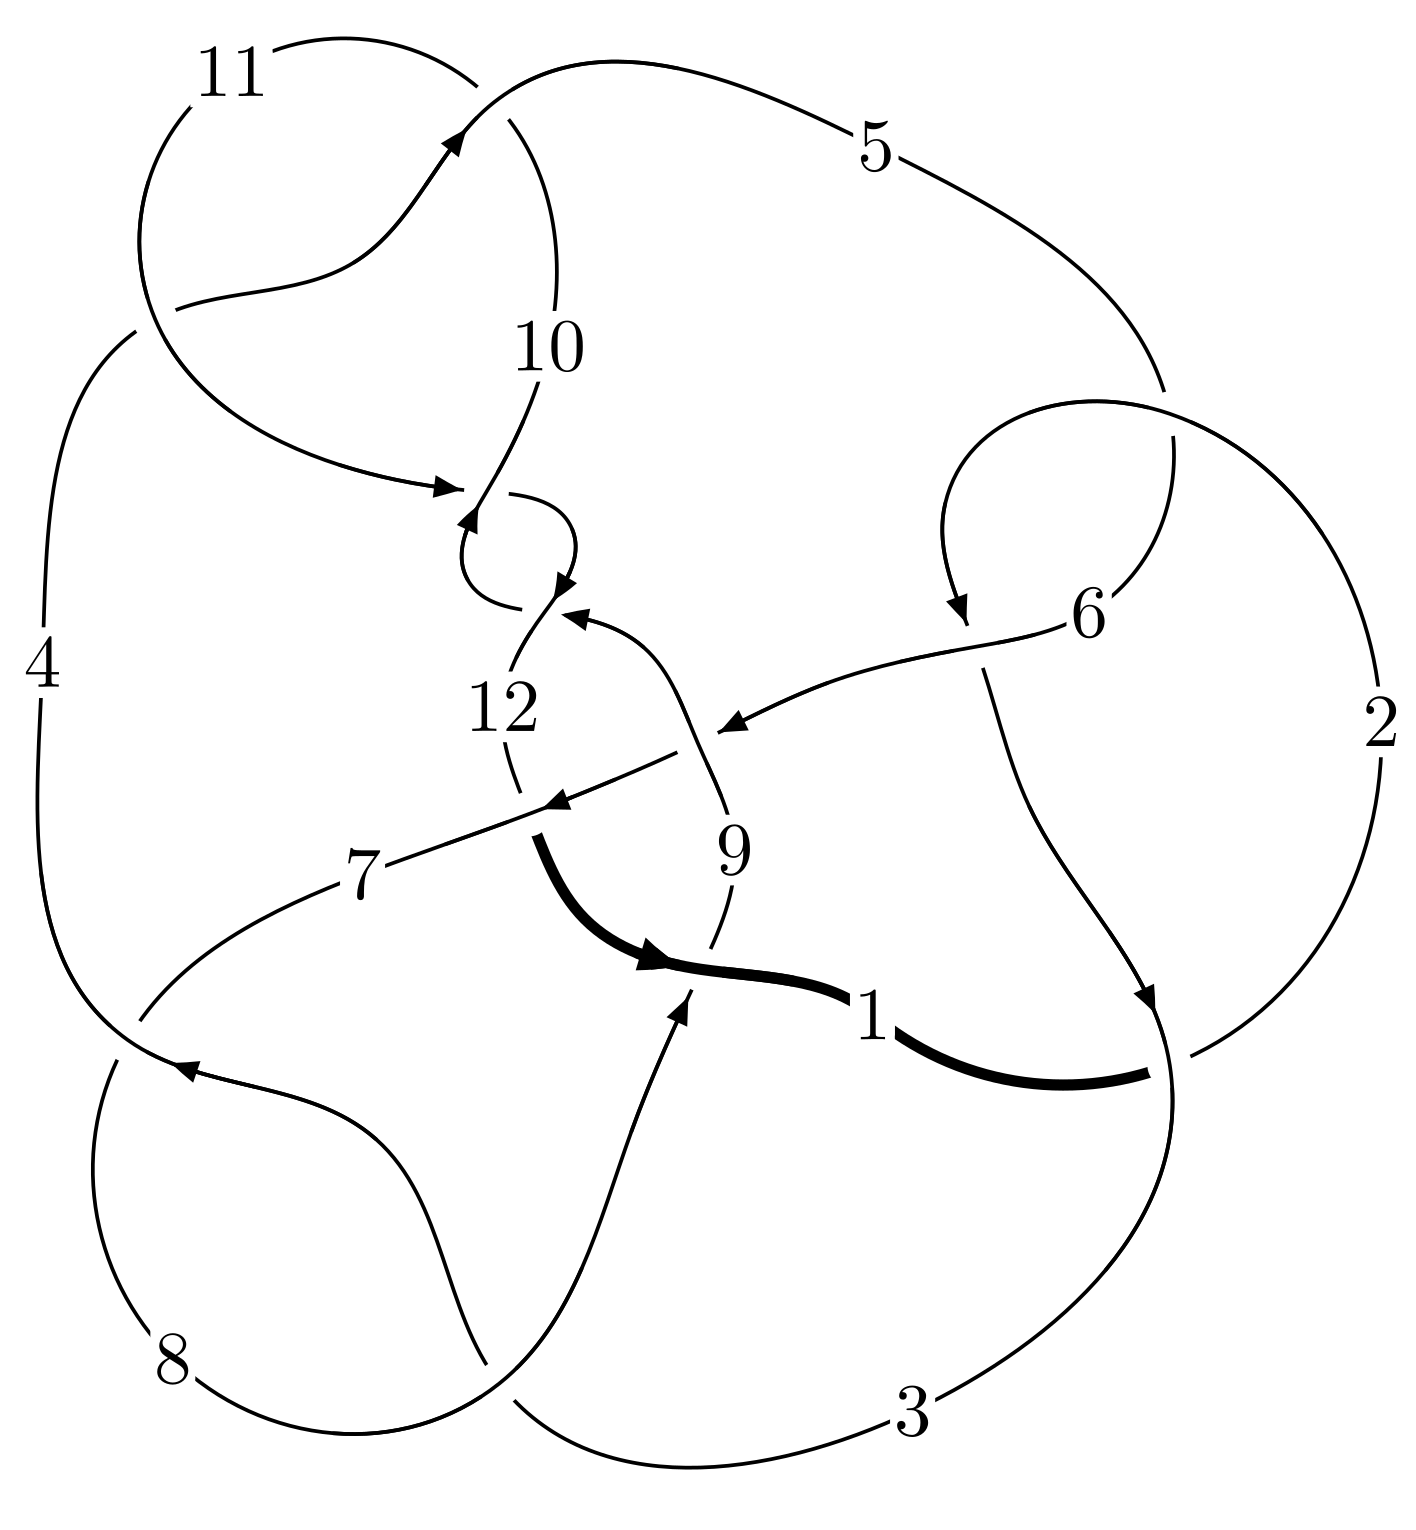
\includegraphics[width=112pt]{../../../GIT/diagram.site/Diagrams/png/1115_12a_0314.png}\\
\ \ \ A knot diagram\footnotemark}&
\allowdisplaybreaks
\textbf{Linearized knot diagam} \\
\cline{2-2}
 &
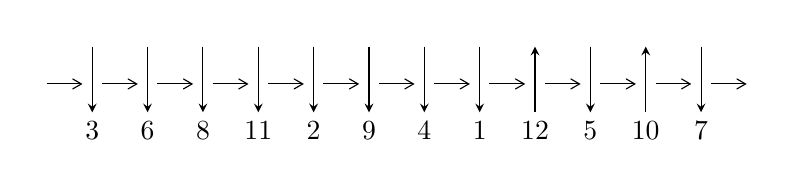
\begin{tikzpicture}[x=20pt, y=17pt]
	% nodes
	\node (C0) at (0, 0) {};
	\node (C1) at (1, 0) {};
	\node (C1U) at (1, +1) {};
	\node (C1D) at (1, -1) {3};

	\node (C2) at (2, 0) {};
	\node (C2U) at (2, +1) {};
	\node (C2D) at (2, -1) {6};

	\node (C3) at (3, 0) {};
	\node (C3U) at (3, +1) {};
	\node (C3D) at (3, -1) {8};

	\node (C4) at (4, 0) {};
	\node (C4U) at (4, +1) {};
	\node (C4D) at (4, -1) {11};

	\node (C5) at (5, 0) {};
	\node (C5U) at (5, +1) {};
	\node (C5D) at (5, -1) {2};

	\node (C6) at (6, 0) {};
	\node (C6U) at (6, +1) {};
	\node (C6D) at (6, -1) {9};

	\node (C7) at (7, 0) {};
	\node (C7U) at (7, +1) {};
	\node (C7D) at (7, -1) {4};

	\node (C8) at (8, 0) {};
	\node (C8U) at (8, +1) {};
	\node (C8D) at (8, -1) {1};

	\node (C9) at (9, 0) {};
	\node (C9U) at (9, +1) {};
	\node (C9D) at (9, -1) {12};

	\node (C10) at (10, 0) {};
	\node (C10U) at (10, +1) {};
	\node (C10D) at (10, -1) {5};

	\node (C11) at (11, 0) {};
	\node (C11U) at (11, +1) {};
	\node (C11D) at (11, -1) {10};

	\node (C12) at (12, 0) {};
	\node (C12U) at (12, +1) {};
	\node (C12D) at (12, -1) {7};
	\node (C13) at (13, 0) {};

	% arrows
	\draw[->,>={angle 60}]
	(C0) edge (C1) (C1) edge (C2) (C2) edge (C3) (C3) edge (C4) (C4) edge (C5) (C5) edge (C6) (C6) edge (C7) (C7) edge (C8) (C8) edge (C9) (C9) edge (C10) (C10) edge (C11) (C11) edge (C12) (C12) edge (C13) ;	\draw[->,>=stealth]
	(C1U) edge (C1D) (C2U) edge (C2D) (C3U) edge (C3D) (C4U) edge (C4D) (C5U) edge (C5D) (C6U) edge (C6D) (C7U) edge (C7D) (C8U) edge (C8D) (C9D) edge (C9U) (C10U) edge (C10D) (C11D) edge (C11U) (C12U) edge (C12D) ;
	\end{tikzpicture} \\
\hhline{~~} \\& 
\textbf{Solving Sequence} \\ \cline{2-2} 
 &
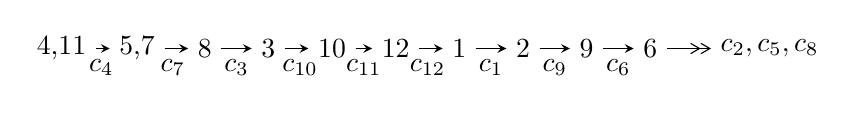
\begin{tikzpicture}[x=23pt, y=7pt]
	% node
	\node (A0) at (-1/8, 0) {4,11};
	\node (A1) at (17/16, 0) {5,7};
	\node (A2) at (17/8, 0) {8};
	\node (A3) at (25/8, 0) {3};
	\node (A4) at (33/8, 0) {10};
	\node (A5) at (41/8, 0) {12};
	\node (A6) at (49/8, 0) {1};
	\node (A7) at (57/8, 0) {2};
	\node (A8) at (65/8, 0) {9};
	\node (A9) at (73/8, 0) {6};
	\node (C1) at (1/2, -1) {$c_{4}$};
	\node (C2) at (13/8, -1) {$c_{7}$};
	\node (C3) at (21/8, -1) {$c_{3}$};
	\node (C4) at (29/8, -1) {$c_{10}$};
	\node (C5) at (37/8, -1) {$c_{11}$};
	\node (C6) at (45/8, -1) {$c_{12}$};
	\node (C7) at (53/8, -1) {$c_{1}$};
	\node (C8) at (61/8, -1) {$c_{9}$};
	\node (C9) at (69/8, -1) {$c_{6}$};
	\node (A10) at (11, 0) {$c_{2},c_{5},c_{8}$};

	% edge
	\draw[->,>=stealth]	
	(A0) edge (A1) (A1) edge (A2) (A2) edge (A3) (A3) edge (A4) (A4) edge (A5) (A5) edge (A6) (A6) edge (A7) (A7) edge (A8) (A8) edge (A9) ;
	\draw[->>,>={angle 60}]	
	(A9) edge (A10);
\end{tikzpicture} \\ 

\end{tabular} \\

\footnotetext{
The image of knot diagram is generated by the software ``\textbf{Draw programme}" developed by Andrew Bartholomew(\url{http://www.layer8.co.uk/maths/draw/index.htm\#Running-draw}), where we modified some parts for our purpose(\url{https://github.com/CATsTAILs/LinksPainter}).
}\phantom \\ \newline 
\centering \textbf{Ideals for irreducible components\footnotemark of $X_{\text{par}}$} 
 
\begin{align*}
I^u_{1}&=\langle 
3.08859\times10^{177} u^{134}+4.12913\times10^{177} u^{133}+\cdots+2.92373\times10^{177} b-6.46265\times10^{177},\\
\phantom{I^u_{1}}&\phantom{= \langle  }-5.20487\times10^{177} u^{134}-7.50538\times10^{177} u^{133}+\cdots+2.92373\times10^{177} a-2.04516\times10^{178},\\
\phantom{I^u_{1}}&\phantom{= \langle  }u^{135}+u^{134}+\cdots-10 u-1\rangle \\
I^u_{2}&=\langle 
- u^{25}-5 u^{23}+\cdots+b+u,\;u^{26}-3 u^{25}+\cdots+a+1,\;u^{27}+6 u^{25}+\cdots+4 u+1\rangle \\
\\
\end{align*}
\raggedright * 2 irreducible components of $\dim_{\mathbb{C}}=0$, with total 162 representations.\\
\footnotetext{All coefficients of polynomials are rational numbers. But the coefficients are sometimes approximated in decimal forms when there is not enough margin.}
\newpage
\renewcommand{\arraystretch}{1}
\centering \section*{I. $I^u_{1}= \langle 3.09\times10^{177} u^{134}+4.13\times10^{177} u^{133}+\cdots+2.92\times10^{177} b-6.46\times10^{177},\;-5.20\times10^{177} u^{134}-7.51\times10^{177} u^{133}+\cdots+2.92\times10^{177} a-2.05\times10^{178},\;u^{135}+u^{134}+\cdots-10 u-1 \rangle$}
\flushleft \textbf{(i) Arc colorings}\\
\begin{tabular}{m{7pt} m{180pt} m{7pt} m{180pt} }
\flushright $a_{4}=$&$\begin{pmatrix}1\\0\end{pmatrix}$ \\
\flushright $a_{11}=$&$\begin{pmatrix}0\\u\end{pmatrix}$ \\
\flushright $a_{5}=$&$\begin{pmatrix}1\\u^2\end{pmatrix}$ \\
\flushright $a_{7}=$&$\begin{pmatrix}1.78022 u^{134}+2.56706 u^{133}+\cdots+1.72860 u+6.99504\\-1.05639 u^{134}-1.41228 u^{133}+\cdots+18.8557 u+2.21042\end{pmatrix}$ \\
\flushright $a_{8}=$&$\begin{pmatrix}2.83661 u^{134}+3.97934 u^{133}+\cdots-17.1271 u+4.78462\\-1.05639 u^{134}-1.41228 u^{133}+\cdots+18.8557 u+2.21042\end{pmatrix}$ \\
\flushright $a_{3}=$&$\begin{pmatrix}0.667462 u^{134}+1.65680 u^{133}+\cdots-88.1836 u-9.43511\\0.245974 u^{134}+0.777931 u^{133}+\cdots-18.2752 u-0.373464\end{pmatrix}$ \\
\flushright $a_{10}=$&$\begin{pmatrix}u\\u^3+u\end{pmatrix}$ \\
\flushright $a_{12}=$&$\begin{pmatrix}u^3\\u^5+u^3+u\end{pmatrix}$ \\
\flushright $a_{1}=$&$\begin{pmatrix}-1.83805 u^{134}-0.271778 u^{133}+\cdots-95.8499 u-4.55202\\1.08576 u^{134}+0.642890 u^{133}+\cdots-0.00908748 u+0.935550\end{pmatrix}$ \\
\flushright $a_{2}=$&$\begin{pmatrix}1.69714 u^{134}+2.70494 u^{133}+\cdots+8.51473 u-3.45506\\-0.898715 u^{134}-2.04841 u^{133}+\cdots+5.14031 u-0.604629\end{pmatrix}$ \\
\flushright $a_{9}=$&$\begin{pmatrix}u^5+u\\u^7+u^5+2 u^3+u\end{pmatrix}$ \\
\flushright $a_{6}=$&$\begin{pmatrix}2.94174 u^{134}+4.34609 u^{133}+\cdots-7.34893 u+6.24805\\-1.64723 u^{134}-2.09134 u^{133}+\cdots+23.2895 u+2.65403\end{pmatrix}$\\&\end{tabular}
\flushleft \textbf{(ii) Obstruction class $= -1$}\\~\\
\flushleft \textbf{(iii) Cusp Shapes $= 2.06282 u^{134}+5.04217 u^{133}+\cdots-3.18528 u-6.72246$}\\~\\
\newpage\renewcommand{\arraystretch}{1}
\flushleft \textbf{(iv) u-Polynomials at the component}\newline \\
\begin{tabular}{m{50pt}|m{274pt}}
Crossings & \hspace{64pt}u-Polynomials at each crossing \\
\hline $$\begin{aligned}c_{1}\end{aligned}$$&$\begin{aligned}
&u^{135}+56 u^{134}+\cdots+282415 u+5041
\end{aligned}$\\
\hline $$\begin{aligned}c_{2},c_{5}\end{aligned}$$&$\begin{aligned}
&u^{135}+2 u^{134}+\cdots-183 u+71
\end{aligned}$\\
\hline $$\begin{aligned}c_{3},c_{7}\end{aligned}$$&$\begin{aligned}
&u^{135}+u^{134}+\cdots+14458 u+16279
\end{aligned}$\\
\hline $$\begin{aligned}c_{4},c_{10}\end{aligned}$$&$\begin{aligned}
&u^{135}- u^{134}+\cdots-10 u+1
\end{aligned}$\\
\hline $$\begin{aligned}c_{6}\end{aligned}$$&$\begin{aligned}
&u^{135}-20 u^{134}+\cdots+12813 u+3131
\end{aligned}$\\
\hline $$\begin{aligned}c_{8}\end{aligned}$$&$\begin{aligned}
&u^{135}-12 u^{134}+\cdots-359245 u+99529
\end{aligned}$\\
\hline $$\begin{aligned}c_{9},c_{11}\end{aligned}$$&$\begin{aligned}
&u^{135}-45 u^{134}+\cdots-76 u+1
\end{aligned}$\\
\hline $$\begin{aligned}c_{12}\end{aligned}$$&$\begin{aligned}
&u^{135}+2 u^{134}+\cdots-115 u+457
\end{aligned}$\\
\hline
\end{tabular}\\~\\
\newpage\renewcommand{\arraystretch}{1}
\flushleft \textbf{(v) Riley Polynomials at the component}\newline \\
\begin{tabular}{m{50pt}|m{274pt}}
Crossings & \hspace{64pt}Riley Polynomials at each crossing \\
\hline $$\begin{aligned}c_{1}\end{aligned}$$&$\begin{aligned}
&y^{135}+60 y^{134}+\cdots+2060543075 y-25411681
\end{aligned}$\\
\hline $$\begin{aligned}c_{2},c_{5}\end{aligned}$$&$\begin{aligned}
&y^{135}-56 y^{134}+\cdots+282415 y-5041
\end{aligned}$\\
\hline $$\begin{aligned}c_{3},c_{7}\end{aligned}$$&$\begin{aligned}
&y^{135}+97 y^{134}+\cdots-11715822106 y-265005841
\end{aligned}$\\
\hline $$\begin{aligned}c_{4},c_{10}\end{aligned}$$&$\begin{aligned}
&y^{135}+45 y^{134}+\cdots-76 y-1
\end{aligned}$\\
\hline $$\begin{aligned}c_{6}\end{aligned}$$&$\begin{aligned}
&y^{135}-22 y^{134}+\cdots+518733671 y-9803161
\end{aligned}$\\
\hline $$\begin{aligned}c_{8}\end{aligned}$$&$\begin{aligned}
&y^{135}+26 y^{134}+\cdots-71452162795 y-9906021841
\end{aligned}$\\
\hline $$\begin{aligned}c_{9},c_{11}\end{aligned}$$&$\begin{aligned}
&y^{135}+101 y^{134}+\cdots+1848 y-1
\end{aligned}$\\
\hline $$\begin{aligned}c_{12}\end{aligned}$$&$\begin{aligned}
&y^{135}-10 y^{134}+\cdots+12233405 y-208849
\end{aligned}$\\
\hline
\end{tabular}\\~\\
\newpage\flushleft \textbf{(vi) Complex Volumes and Cusp Shapes}
$$\begin{array}{c|c|c}  
\text{Solutions to }I^u_{1}& \I (\text{vol} + \sqrt{-1}CS) & \text{Cusp shape}\\
 \hline 
\begin{aligned}
u &= \phantom{-}0.182191 + 0.978011 I \\
a &= \phantom{-}0.053526 + 0.498105 I \\
b &= -0.913562 - 0.305391 I\end{aligned}
 & \phantom{-}2.78439 - 2.21481 I & \phantom{-0.000000 } 0 \\ \hline\begin{aligned}
u &= \phantom{-}0.182191 - 0.978011 I \\
a &= \phantom{-}0.053526 - 0.498105 I \\
b &= -0.913562 + 0.305391 I\end{aligned}
 & \phantom{-}2.78439 + 2.21481 I & \phantom{-0.000000 } 0 \\ \hline\begin{aligned}
u &= -0.257952 + 0.978394 I \\
a &= -0.207563 + 0.191828 I \\
b &= \phantom{-}1.040760 - 0.132048 I\end{aligned}
 & \phantom{-}1.69152 + 7.21546 I & \phantom{-0.000000 } 0 \\ \hline\begin{aligned}
u &= -0.257952 - 0.978394 I \\
a &= -0.207563 - 0.191828 I \\
b &= \phantom{-}1.040760 + 0.132048 I\end{aligned}
 & \phantom{-}1.69152 - 7.21546 I & \phantom{-0.000000 } 0 \\ \hline\begin{aligned}
u &= \phantom{-}0.297927 + 0.935277 I \\
a &= \phantom{-}0.554906 + 0.972744 I \\
b &= -0.375896 + 0.194038 I\end{aligned}
 & \phantom{-}2.04642 - 3.11861 I & \phantom{-0.000000 } 0 \\ \hline\begin{aligned}
u &= \phantom{-}0.297927 - 0.935277 I \\
a &= \phantom{-}0.554906 - 0.972744 I \\
b &= -0.375896 - 0.194038 I\end{aligned}
 & \phantom{-}2.04642 + 3.11861 I & \phantom{-0.000000 } 0 \\ \hline\begin{aligned}
u &= \phantom{-}0.048541 + 1.020490 I \\
a &= -0.281366 + 0.850989 I \\
b &= -0.229769 - 0.550795 I\end{aligned}
 & \phantom{-}2.37651 - 1.33885 I & \phantom{-0.000000 } 0 \\ \hline\begin{aligned}
u &= \phantom{-}0.048541 - 1.020490 I \\
a &= -0.281366 - 0.850989 I \\
b &= -0.229769 + 0.550795 I\end{aligned}
 & \phantom{-}2.37651 + 1.33885 I & \phantom{-0.000000 } 0 \\ \hline\begin{aligned}
u &= \phantom{-}0.624839 + 0.743352 I \\
a &= \phantom{-}1.36143 + 0.58880 I \\
b &= \phantom{-}0.33558 + 1.44289 I\end{aligned}
 & \phantom{-}1.44939 - 4.62743 I & \phantom{-0.000000 } 0 \\ \hline\begin{aligned}
u &= \phantom{-}0.624839 - 0.743352 I \\
a &= \phantom{-}1.36143 - 0.58880 I \\
b &= \phantom{-}0.33558 - 1.44289 I\end{aligned}
 & \phantom{-}1.44939 + 4.62743 I & \phantom{-0.000000 } 0\\
 \hline 
 \end{array}$$\newpage$$\begin{array}{c|c|c}  
\text{Solutions to }I^u_{1}& \I (\text{vol} + \sqrt{-1}CS) & \text{Cusp shape}\\
 \hline 
\begin{aligned}
u &= -0.687698 + 0.766698 I \\
a &= \phantom{-}1.22927 + 1.70192 I \\
b &= \phantom{-}0.93164 + 1.16301 I\end{aligned}
 & \phantom{-}1.08282 - 3.99338 I & \phantom{-0.000000 } 0 \\ \hline\begin{aligned}
u &= -0.687698 - 0.766698 I \\
a &= \phantom{-}1.22927 - 1.70192 I \\
b &= \phantom{-}0.93164 - 1.16301 I\end{aligned}
 & \phantom{-}1.08282 + 3.99338 I & \phantom{-0.000000 } 0 \\ \hline\begin{aligned}
u &= \phantom{-}0.322455 + 0.986690 I \\
a &= \phantom{-}1.30133 - 0.65999 I \\
b &= \phantom{-}0.288260 + 1.111700 I\end{aligned}
 & \phantom{-}1.00007 - 5.31249 I & \phantom{-0.000000 } 0 \\ \hline\begin{aligned}
u &= \phantom{-}0.322455 - 0.986690 I \\
a &= \phantom{-}1.30133 + 0.65999 I \\
b &= \phantom{-}0.288260 - 1.111700 I\end{aligned}
 & \phantom{-}1.00007 + 5.31249 I & \phantom{-0.000000 } 0 \\ \hline\begin{aligned}
u &= -0.784066 + 0.556358 I \\
a &= \phantom{-}0.394134 - 0.253532 I \\
b &= \phantom{-}0.030061 + 0.779063 I\end{aligned}
 & -3.06388 + 0.25442 I & \phantom{-0.000000 } 0 \\ \hline\begin{aligned}
u &= -0.784066 - 0.556358 I \\
a &= \phantom{-}0.394134 + 0.253532 I \\
b &= \phantom{-}0.030061 - 0.779063 I\end{aligned}
 & -3.06388 - 0.25442 I & \phantom{-0.000000 } 0 \\ \hline\begin{aligned}
u &= \phantom{-}0.017373 + 0.959928 I \\
a &= -0.26438 + 1.69451 I \\
b &= -0.66691 - 1.45421 I\end{aligned}
 & \phantom{-}5.75111 - 4.49804 I & \phantom{-0.000000 } 0 \\ \hline\begin{aligned}
u &= \phantom{-}0.017373 - 0.959928 I \\
a &= -0.26438 - 1.69451 I \\
b &= -0.66691 + 1.45421 I\end{aligned}
 & \phantom{-}5.75111 + 4.49804 I & \phantom{-0.000000 } 0 \\ \hline\begin{aligned}
u &= \phantom{-}0.690019 + 0.794749 I \\
a &= -0.70119 + 1.83083 I \\
b &= -0.733382 + 1.200060 I\end{aligned}
 & \phantom{-}1.64624 - 1.58894 I & \phantom{-0.000000 } 0 \\ \hline\begin{aligned}
u &= \phantom{-}0.690019 - 0.794749 I \\
a &= -0.70119 - 1.83083 I \\
b &= -0.733382 - 1.200060 I\end{aligned}
 & \phantom{-}1.64624 + 1.58894 I & \phantom{-0.000000 } 0\\
 \hline 
 \end{array}$$\newpage$$\begin{array}{c|c|c}  
\text{Solutions to }I^u_{1}& \I (\text{vol} + \sqrt{-1}CS) & \text{Cusp shape}\\
 \hline 
\begin{aligned}
u &= -0.124250 + 1.052510 I \\
a &= -0.374282 + 1.019370 I \\
b &= \phantom{-}0.242021 - 0.356502 I\end{aligned}
 & \phantom{-}2.47481 - 1.46151 I & \phantom{-0.000000 } 0 \\ \hline\begin{aligned}
u &= -0.124250 - 1.052510 I \\
a &= -0.374282 - 1.019370 I \\
b &= \phantom{-}0.242021 + 0.356502 I\end{aligned}
 & \phantom{-}2.47481 + 1.46151 I & \phantom{-0.000000 } 0 \\ \hline\begin{aligned}
u &= \phantom{-}0.730207 + 0.768827 I \\
a &= \phantom{-}1.38692 - 0.88175 I \\
b &= \phantom{-}0.083254 - 1.033660 I\end{aligned}
 & \phantom{-}1.61638 + 0.94446 I & \phantom{-0.000000 } 0 \\ \hline\begin{aligned}
u &= \phantom{-}0.730207 - 0.768827 I \\
a &= \phantom{-}1.38692 + 0.88175 I \\
b &= \phantom{-}0.083254 + 1.033660 I\end{aligned}
 & \phantom{-}1.61638 - 0.94446 I & \phantom{-0.000000 } 0 \\ \hline\begin{aligned}
u &= -0.672932 + 0.819553 I \\
a &= -1.43281 - 0.80589 I \\
b &= \phantom{-}0.040967 - 0.796293 I\end{aligned}
 & \phantom{-}0.78023 + 5.76542 I & \phantom{-0.000000 } 0 \\ \hline\begin{aligned}
u &= -0.672932 - 0.819553 I \\
a &= -1.43281 + 0.80589 I \\
b &= \phantom{-}0.040967 + 0.796293 I\end{aligned}
 & \phantom{-}0.78023 - 5.76542 I & \phantom{-0.000000 } 0 \\ \hline\begin{aligned}
u &= -0.781702 + 0.719098 I \\
a &= \phantom{-}1.184710 + 0.338601 I \\
b &= \phantom{-}0.786645 + 0.475694 I\end{aligned}
 & -3.44393 - 1.01362 I & \phantom{-0.000000 } 0 \\ \hline\begin{aligned}
u &= -0.781702 - 0.719098 I \\
a &= \phantom{-}1.184710 - 0.338601 I \\
b &= \phantom{-}0.786645 - 0.475694 I\end{aligned}
 & -3.44393 + 1.01362 I & \phantom{-0.000000 } 0 \\ \hline\begin{aligned}
u &= -0.073144 + 0.932715 I \\
a &= -2.00962 - 2.39100 I \\
b &= -0.051227 + 1.230250 I\end{aligned}
 & \phantom{-}6.80128 + 1.87487 I & \phantom{-0.000000 } 0 \\ \hline\begin{aligned}
u &= -0.073144 - 0.932715 I \\
a &= -2.00962 + 2.39100 I \\
b &= -0.051227 - 1.230250 I\end{aligned}
 & \phantom{-}6.80128 - 1.87487 I & \phantom{-0.000000 } 0\\
 \hline 
 \end{array}$$\newpage$$\begin{array}{c|c|c}  
\text{Solutions to }I^u_{1}& \I (\text{vol} + \sqrt{-1}CS) & \text{Cusp shape}\\
 \hline 
\begin{aligned}
u &= \phantom{-}0.886558 + 0.603387 I \\
a &= -0.355164 + 0.151303 I \\
b &= -0.296286 + 1.079330 I\end{aligned}
 & -3.81694 + 3.79135 I & \phantom{-0.000000 } 0 \\ \hline\begin{aligned}
u &= \phantom{-}0.886558 - 0.603387 I \\
a &= -0.355164 - 0.151303 I \\
b &= -0.296286 - 1.079330 I\end{aligned}
 & -3.81694 - 3.79135 I & \phantom{-0.000000 } 0 \\ \hline\begin{aligned}
u &= \phantom{-}0.721149 + 0.797335 I \\
a &= \phantom{-}0.206670 + 0.515003 I \\
b &= \phantom{-}0.241979 - 1.324930 I\end{aligned}
 & \phantom{-}0.03808 + 3.51542 I & \phantom{-0.000000 } 0 \\ \hline\begin{aligned}
u &= \phantom{-}0.721149 - 0.797335 I \\
a &= \phantom{-}0.206670 - 0.515003 I \\
b &= \phantom{-}0.241979 + 1.324930 I\end{aligned}
 & \phantom{-}0.03808 - 3.51542 I & \phantom{-0.000000 } 0 \\ \hline\begin{aligned}
u &= -0.712957 + 0.814314 I \\
a &= -1.33242 + 0.66330 I \\
b &= -0.18819 + 1.77652 I\end{aligned}
 & \phantom{-}1.68930 + 0.74766 I & \phantom{-0.000000 } 0 \\ \hline\begin{aligned}
u &= -0.712957 - 0.814314 I \\
a &= -1.33242 - 0.66330 I \\
b &= -0.18819 - 1.77652 I\end{aligned}
 & \phantom{-}1.68930 - 0.74766 I & \phantom{-0.000000 } 0 \\ \hline\begin{aligned}
u &= -0.801154 + 0.742049 I \\
a &= \phantom{-}1.55777 + 0.32439 I \\
b &= \phantom{-}1.060750 + 0.043144 I\end{aligned}
 & -3.59680 - 1.35599 I & \phantom{-0.000000 } 0 \\ \hline\begin{aligned}
u &= -0.801154 - 0.742049 I \\
a &= \phantom{-}1.55777 - 0.32439 I \\
b &= \phantom{-}1.060750 - 0.043144 I\end{aligned}
 & -3.59680 + 1.35599 I & \phantom{-0.000000 } 0 \\ \hline\begin{aligned}
u &= -0.650109 + 0.880076 I \\
a &= \phantom{-}0.84298 + 1.23027 I \\
b &= -0.014753 - 1.331240 I\end{aligned}
 & \phantom{-}3.78897 + 2.52031 I & \phantom{-0.000000 } 0 \\ \hline\begin{aligned}
u &= -0.650109 - 0.880076 I \\
a &= \phantom{-}0.84298 - 1.23027 I \\
b &= -0.014753 + 1.331240 I\end{aligned}
 & \phantom{-}3.78897 - 2.52031 I & \phantom{-0.000000 } 0\\
 \hline 
 \end{array}$$\newpage$$\begin{array}{c|c|c}  
\text{Solutions to }I^u_{1}& \I (\text{vol} + \sqrt{-1}CS) & \text{Cusp shape}\\
 \hline 
\begin{aligned}
u &= -0.028887 + 0.899858 I \\
a &= \phantom{-}1.42340 - 3.31692 I \\
b &= -0.128305 + 1.165830 I\end{aligned}
 & \phantom{-}4.74784 + 4.74110 I & \phantom{-0.000000 } 0 \\ \hline\begin{aligned}
u &= -0.028887 - 0.899858 I \\
a &= \phantom{-}1.42340 + 3.31692 I \\
b &= -0.128305 - 1.165830 I\end{aligned}
 & \phantom{-}4.74784 - 4.74110 I & \phantom{-0.000000 } 0 \\ \hline\begin{aligned}
u &= -0.002396 + 0.896636 I \\
a &= \phantom{-}0.60825 + 1.82878 I \\
b &= \phantom{-}0.48954 - 1.57452 I\end{aligned}
 & \phantom{-}6.04754 - 0.54483 I & \phantom{-0.000000 } 0 \\ \hline\begin{aligned}
u &= -0.002396 - 0.896636 I \\
a &= \phantom{-}0.60825 - 1.82878 I \\
b &= \phantom{-}0.48954 + 1.57452 I\end{aligned}
 & \phantom{-}6.04754 + 0.54483 I & \phantom{-0.000000 } 0 \\ \hline\begin{aligned}
u &= \phantom{-}0.863693 + 0.692591 I \\
a &= \phantom{-}0.897732 - 0.804504 I \\
b &= \phantom{-}0.52708 - 1.32870 I\end{aligned}
 & \phantom{-}0.56808 + 6.92229 I & \phantom{-0.000000 } 0 \\ \hline\begin{aligned}
u &= \phantom{-}0.863693 - 0.692591 I \\
a &= \phantom{-}0.897732 + 0.804504 I \\
b &= \phantom{-}0.52708 + 1.32870 I\end{aligned}
 & \phantom{-}0.56808 - 6.92229 I & \phantom{-0.000000 } 0 \\ \hline\begin{aligned}
u &= -0.894065 + 0.688028 I \\
a &= -0.840171 - 0.806541 I \\
b &= -0.65417 - 1.37472 I\end{aligned}
 & -1.49753 - 12.96880 I & \phantom{-0.000000 } 0 \\ \hline\begin{aligned}
u &= -0.894065 - 0.688028 I \\
a &= -0.840171 + 0.806541 I \\
b &= -0.65417 + 1.37472 I\end{aligned}
 & -1.49753 + 12.96880 I & \phantom{-0.000000 } 0 \\ \hline\begin{aligned}
u &= -0.197669 + 1.111950 I \\
a &= -0.88725 - 1.44321 I \\
b &= -0.403719 + 1.351080 I\end{aligned}
 & \phantom{-}7.76949 + 6.79943 I & \phantom{-0.000000 } 0 \\ \hline\begin{aligned}
u &= -0.197669 - 1.111950 I \\
a &= -0.88725 + 1.44321 I \\
b &= -0.403719 - 1.351080 I\end{aligned}
 & \phantom{-}7.76949 - 6.79943 I & \phantom{-0.000000 } 0\\
 \hline 
 \end{array}$$\newpage$$\begin{array}{c|c|c}  
\text{Solutions to }I^u_{1}& \I (\text{vol} + \sqrt{-1}CS) & \text{Cusp shape}\\
 \hline 
\begin{aligned}
u &= \phantom{-}0.840905 + 0.754988 I \\
a &= -1.65520 + 0.40132 I \\
b &= -1.346250 - 0.168487 I\end{aligned}
 & -5.37206 + 6.09957 I & \phantom{-0.000000 } 0 \\ \hline\begin{aligned}
u &= \phantom{-}0.840905 - 0.754988 I \\
a &= -1.65520 - 0.40132 I \\
b &= -1.346250 + 0.168487 I\end{aligned}
 & -5.37206 - 6.09957 I & \phantom{-0.000000 } 0 \\ \hline\begin{aligned}
u &= \phantom{-}0.851238 + 0.147950 I \\
a &= -0.718097 - 0.554840 I \\
b &= -0.530662 - 1.202540 I\end{aligned}
 & \phantom{-}1.65967 - 9.19748 I & \phantom{-0.000000 } 0 \\ \hline\begin{aligned}
u &= \phantom{-}0.851238 - 0.147950 I \\
a &= -0.718097 + 0.554840 I \\
b &= -0.530662 + 1.202540 I\end{aligned}
 & \phantom{-}1.65967 + 9.19748 I & \phantom{-0.000000 } 0 \\ \hline\begin{aligned}
u &= -0.681150 + 0.910444 I \\
a &= \phantom{-}2.83794 - 0.14278 I \\
b &= \phantom{-}0.011720 - 0.931068 I\end{aligned}
 & \phantom{-}1.066200 - 0.522589 I & \phantom{-0.000000 } 0 \\ \hline\begin{aligned}
u &= -0.681150 - 0.910444 I \\
a &= \phantom{-}2.83794 + 0.14278 I \\
b &= \phantom{-}0.011720 + 0.931068 I\end{aligned}
 & \phantom{-}1.066200 + 0.522589 I & \phantom{-0.000000 } 0 \\ \hline\begin{aligned}
u &= \phantom{-}0.793490 + 0.819836 I \\
a &= -1.84178 + 0.28996 I \\
b &= -0.869259 - 0.565594 I\end{aligned}
 & -7.86699 - 0.96280 I & \phantom{-0.000000 } 0 \\ \hline\begin{aligned}
u &= \phantom{-}0.793490 - 0.819836 I \\
a &= -1.84178 - 0.28996 I \\
b &= -0.869259 + 0.565594 I\end{aligned}
 & -7.86699 + 0.96280 I & \phantom{-0.000000 } 0 \\ \hline\begin{aligned}
u &= \phantom{-}0.876571 + 0.732191 I \\
a &= -0.611541 + 0.448689 I \\
b &= -0.745897 + 0.893684 I\end{aligned}
 & -4.74494 - 1.40898 I & \phantom{-0.000000 } 0 \\ \hline\begin{aligned}
u &= \phantom{-}0.876571 - 0.732191 I \\
a &= -0.611541 - 0.448689 I \\
b &= -0.745897 - 0.893684 I\end{aligned}
 & -4.74494 + 1.40898 I & \phantom{-0.000000 } 0\\
 \hline 
 \end{array}$$\newpage$$\begin{array}{c|c|c}  
\text{Solutions to }I^u_{1}& \I (\text{vol} + \sqrt{-1}CS) & \text{Cusp shape}\\
 \hline 
\begin{aligned}
u &= \phantom{-}0.790320 + 0.825636 I \\
a &= \phantom{-}0.961027 + 0.336341 I \\
b &= \phantom{-}0.329707 + 0.756995 I\end{aligned}
 & -2.17948 - 2.71087 I & \phantom{-0.000000 } 0 \\ \hline\begin{aligned}
u &= \phantom{-}0.790320 - 0.825636 I \\
a &= \phantom{-}0.961027 - 0.336341 I \\
b &= \phantom{-}0.329707 - 0.756995 I\end{aligned}
 & -2.17948 + 2.71087 I & \phantom{-0.000000 } 0 \\ \hline\begin{aligned}
u &= -0.852083 + 0.765794 I \\
a &= -0.894156 - 0.987576 I \\
b &= -0.486242 - 1.010700 I\end{aligned}
 & -6.42768 - 3.99066 I & \phantom{-0.000000 } 0 \\ \hline\begin{aligned}
u &= -0.852083 - 0.765794 I \\
a &= -0.894156 + 0.987576 I \\
b &= -0.486242 + 1.010700 I\end{aligned}
 & -6.42768 + 3.99066 I & \phantom{-0.000000 } 0 \\ \hline\begin{aligned}
u &= \phantom{-}0.655478 + 0.942520 I \\
a &= \phantom{-}1.152080 + 0.765922 I \\
b &= -0.40671 + 1.56053 I\end{aligned}
 & \phantom{-}2.05184 - 0.42331 I & \phantom{-0.000000 } 0 \\ \hline\begin{aligned}
u &= \phantom{-}0.655478 - 0.942520 I \\
a &= \phantom{-}1.152080 - 0.765922 I \\
b &= -0.40671 - 1.56053 I\end{aligned}
 & \phantom{-}2.05184 + 0.42331 I & \phantom{-0.000000 } 0 \\ \hline\begin{aligned}
u &= \phantom{-}0.689876 + 0.924925 I \\
a &= \phantom{-}2.63892 + 0.23797 I \\
b &= \phantom{-}0.76308 + 1.35140 I\end{aligned}
 & \phantom{-}2.04503 - 3.73553 I & \phantom{-0.000000 } 0 \\ \hline\begin{aligned}
u &= \phantom{-}0.689876 - 0.924925 I \\
a &= \phantom{-}2.63892 - 0.23797 I \\
b &= \phantom{-}0.76308 - 1.35140 I\end{aligned}
 & \phantom{-}2.04503 + 3.73553 I & \phantom{-0.000000 } 0 \\ \hline\begin{aligned}
u &= -0.702748 + 0.919564 I \\
a &= -1.24798 + 0.76455 I \\
b &= \phantom{-}0.28362 + 1.80278 I\end{aligned}
 & \phantom{-}2.01595 + 4.68054 I & \phantom{-0.000000 } 0 \\ \hline\begin{aligned}
u &= -0.702748 - 0.919564 I \\
a &= -1.24798 - 0.76455 I \\
b &= \phantom{-}0.28362 - 1.80278 I\end{aligned}
 & \phantom{-}2.01595 - 4.68054 I & \phantom{-0.000000 } 0\\
 \hline 
 \end{array}$$\newpage$$\begin{array}{c|c|c}  
\text{Solutions to }I^u_{1}& \I (\text{vol} + \sqrt{-1}CS) & \text{Cusp shape}\\
 \hline 
\begin{aligned}
u &= -0.884733 + 0.752880 I \\
a &= -0.531180 + 0.206844 I \\
b &= -0.200453 + 0.496698 I\end{aligned}
 & -5.74291 - 1.34202 I & \phantom{-0.000000 } 0 \\ \hline\begin{aligned}
u &= -0.884733 - 0.752880 I \\
a &= -0.531180 - 0.206844 I \\
b &= -0.200453 - 0.496698 I\end{aligned}
 & -5.74291 + 1.34202 I & \phantom{-0.000000 } 0 \\ \hline\begin{aligned}
u &= \phantom{-}0.158242 + 1.155000 I \\
a &= -0.349033 + 0.640872 I \\
b &= \phantom{-}0.028732 - 0.815651 I\end{aligned}
 & \phantom{-}2.19994 - 1.27262 I & \phantom{-0.000000 } 0 \\ \hline\begin{aligned}
u &= \phantom{-}0.158242 - 1.155000 I \\
a &= -0.349033 - 0.640872 I \\
b &= \phantom{-}0.028732 + 0.815651 I\end{aligned}
 & \phantom{-}2.19994 + 1.27262 I & \phantom{-0.000000 } 0 \\ \hline\begin{aligned}
u &= -0.684601 + 0.945585 I \\
a &= -2.77824 - 0.26400 I \\
b &= -0.94746 + 1.30952 I\end{aligned}
 & \phantom{-}1.63233 + 9.30140 I & \phantom{-0.000000 } 0 \\ \hline\begin{aligned}
u &= -0.684601 - 0.945585 I \\
a &= -2.77824 + 0.26400 I \\
b &= -0.94746 - 1.30952 I\end{aligned}
 & \phantom{-}1.63233 - 9.30140 I & \phantom{-0.000000 } 0 \\ \hline\begin{aligned}
u &= \phantom{-}0.706799 + 0.930995 I \\
a &= -1.69494 + 1.17271 I \\
b &= -0.194351 - 1.328060 I\end{aligned}
 & \phantom{-}0.44874 - 8.98252 I & \phantom{-0.000000 } 0 \\ \hline\begin{aligned}
u &= \phantom{-}0.706799 - 0.930995 I \\
a &= -1.69494 - 1.17271 I \\
b &= -0.194351 + 1.328060 I\end{aligned}
 & \phantom{-}0.44874 + 8.98252 I & \phantom{-0.000000 } 0 \\ \hline\begin{aligned}
u &= \phantom{-}0.221920 + 1.151170 I \\
a &= \phantom{-}0.69674 - 1.35373 I \\
b &= \phantom{-}0.51132 + 1.34118 I\end{aligned}
 & \phantom{-}6.10373 - 12.62740 I & \phantom{-0.000000 } 0 \\ \hline\begin{aligned}
u &= \phantom{-}0.221920 - 1.151170 I \\
a &= \phantom{-}0.69674 + 1.35373 I \\
b &= \phantom{-}0.51132 - 1.34118 I\end{aligned}
 & \phantom{-}6.10373 + 12.62740 I & \phantom{-0.000000 } 0\\
 \hline 
 \end{array}$$\newpage$$\begin{array}{c|c|c}  
\text{Solutions to }I^u_{1}& \I (\text{vol} + \sqrt{-1}CS) & \text{Cusp shape}\\
 \hline 
\begin{aligned}
u &= -0.437000 + 1.100790 I \\
a &= \phantom{-}0.864126 + 0.513330 I \\
b &= -0.264139 - 1.258760 I\end{aligned}
 & \phantom{-}6.37212 + 0.50399 I & \phantom{-0.000000 } 0 \\ \hline\begin{aligned}
u &= -0.437000 - 1.100790 I \\
a &= \phantom{-}0.864126 - 0.513330 I \\
b &= -0.264139 + 1.258760 I\end{aligned}
 & \phantom{-}6.37212 - 0.50399 I & \phantom{-0.000000 } 0 \\ \hline\begin{aligned}
u &= \phantom{-}0.708667 + 0.949566 I \\
a &= -2.83413 - 0.15041 I \\
b &= -0.128903 - 1.089500 I\end{aligned}
 & \phantom{-}2.16540 - 6.44695 I & \phantom{-0.000000 } 0 \\ \hline\begin{aligned}
u &= \phantom{-}0.708667 - 0.949566 I \\
a &= -2.83413 + 0.15041 I \\
b &= -0.128903 + 1.089500 I\end{aligned}
 & \phantom{-}2.16540 + 6.44695 I & \phantom{-0.000000 } 0 \\ \hline\begin{aligned}
u &= \phantom{-}0.741269 + 0.929721 I \\
a &= -0.056422 + 0.467169 I \\
b &= -0.332085 + 0.578033 I\end{aligned}
 & -1.85034 - 3.06303 I & \phantom{-0.000000 } 0 \\ \hline\begin{aligned}
u &= \phantom{-}0.741269 - 0.929721 I \\
a &= -0.056422 - 0.467169 I \\
b &= -0.332085 - 0.578033 I\end{aligned}
 & -1.85034 + 3.06303 I & \phantom{-0.000000 } 0 \\ \hline\begin{aligned}
u &= -0.198998 + 0.780233 I \\
a &= \phantom{-}0.716435 + 0.210614 I \\
b &= \phantom{-}0.764763 + 0.174582 I\end{aligned}
 & -1.97377 + 1.53826 I & \phantom{-0.000000 } 0 \\ \hline\begin{aligned}
u &= -0.198998 - 0.780233 I \\
a &= \phantom{-}0.716435 - 0.210614 I \\
b &= \phantom{-}0.764763 - 0.174582 I\end{aligned}
 & -1.97377 - 1.53826 I & \phantom{-0.000000 } 0 \\ \hline\begin{aligned}
u &= \phantom{-}0.760414 + 0.933967 I \\
a &= \phantom{-}1.058620 - 0.882520 I \\
b &= \phantom{-}0.928936 - 0.502379 I\end{aligned}
 & -7.51384 - 4.88368 I & \phantom{-0.000000 } 0 \\ \hline\begin{aligned}
u &= \phantom{-}0.760414 - 0.933967 I \\
a &= \phantom{-}1.058620 + 0.882520 I \\
b &= \phantom{-}0.928936 + 0.502379 I\end{aligned}
 & -7.51384 + 4.88368 I & \phantom{-0.000000 } 0\\
 \hline 
 \end{array}$$\newpage$$\begin{array}{c|c|c}  
\text{Solutions to }I^u_{1}& \I (\text{vol} + \sqrt{-1}CS) & \text{Cusp shape}\\
 \hline 
\begin{aligned}
u &= -0.826433 + 0.884407 I \\
a &= \phantom{-}0.502926 + 0.497730 I \\
b &= \phantom{-}0.716200 + 0.483626 I\end{aligned}
 & -5.32606 - 0.60628 I & \phantom{-0.000000 } 0 \\ \hline\begin{aligned}
u &= -0.826433 - 0.884407 I \\
a &= \phantom{-}0.502926 - 0.497730 I \\
b &= \phantom{-}0.716200 - 0.483626 I\end{aligned}
 & -5.32606 + 0.60628 I & \phantom{-0.000000 } 0 \\ \hline\begin{aligned}
u &= -0.762596 + 0.167367 I \\
a &= \phantom{-}0.796811 - 0.619266 I \\
b &= \phantom{-}0.374725 - 1.239250 I\end{aligned}
 & \phantom{-}3.51291 + 3.79183 I & -8.00000 - 3.66278 I \\ \hline\begin{aligned}
u &= -0.762596 - 0.167367 I \\
a &= \phantom{-}0.796811 + 0.619266 I \\
b &= \phantom{-}0.374725 + 1.239250 I\end{aligned}
 & \phantom{-}3.51291 - 3.79183 I & -8.00000 + 3.66278 I \\ \hline\begin{aligned}
u &= -0.717460 + 0.991265 I \\
a &= -1.61017 - 0.78407 I \\
b &= -0.785319 + 0.609006 I\end{aligned}
 & -2.61535 + 6.68659 I & \phantom{-0.000000 } 0 \\ \hline\begin{aligned}
u &= -0.717460 - 0.991265 I \\
a &= -1.61017 + 0.78407 I \\
b &= -0.785319 - 0.609006 I\end{aligned}
 & -2.61535 - 6.68659 I & \phantom{-0.000000 } 0 \\ \hline\begin{aligned}
u &= -0.737356 + 0.983139 I \\
a &= -1.34639 - 1.08442 I \\
b &= -1.122400 + 0.095325 I\end{aligned}
 & -2.86184 + 7.14763 I & \phantom{-0.000000 } 0 \\ \hline\begin{aligned}
u &= -0.737356 - 0.983139 I \\
a &= -1.34639 + 1.08442 I \\
b &= -1.122400 - 0.095325 I\end{aligned}
 & -2.86184 - 7.14763 I & \phantom{-0.000000 } 0 \\ \hline\begin{aligned}
u &= -0.025837 + 1.233540 I \\
a &= -0.059316 + 1.259640 I \\
b &= \phantom{-}0.106338 - 1.025650 I\end{aligned}
 & \phantom{-}2.97005 + 2.13809 I & \phantom{-0.000000 } 0 \\ \hline\begin{aligned}
u &= -0.025837 - 1.233540 I \\
a &= -0.059316 - 1.259640 I \\
b &= \phantom{-}0.106338 + 1.025650 I\end{aligned}
 & \phantom{-}2.97005 - 2.13809 I & \phantom{-0.000000 } 0\\
 \hline 
 \end{array}$$\newpage$$\begin{array}{c|c|c}  
\text{Solutions to }I^u_{1}& \I (\text{vol} + \sqrt{-1}CS) & \text{Cusp shape}\\
 \hline 
\begin{aligned}
u &= -0.847510 + 0.896957 I \\
a &= -1.069150 - 0.156979 I \\
b &= -0.667049 + 0.655089 I\end{aligned}
 & -5.30570 + 6.81308 I & \phantom{-0.000000 } 0 \\ \hline\begin{aligned}
u &= -0.847510 - 0.896957 I \\
a &= -1.069150 + 0.156979 I \\
b &= -0.667049 - 0.655089 I\end{aligned}
 & -5.30570 - 6.81308 I & \phantom{-0.000000 } 0 \\ \hline\begin{aligned}
u &= \phantom{-}0.417407 + 1.173910 I \\
a &= -0.785299 + 0.387509 I \\
b &= \phantom{-}0.387239 - 1.149160 I\end{aligned}
 & \phantom{-}4.97232 + 4.61880 I & \phantom{-0.000000 } 0 \\ \hline\begin{aligned}
u &= \phantom{-}0.417407 - 1.173910 I \\
a &= -0.785299 - 0.387509 I \\
b &= \phantom{-}0.387239 + 1.149160 I\end{aligned}
 & \phantom{-}4.97232 - 4.61880 I & \phantom{-0.000000 } 0 \\ \hline\begin{aligned}
u &= -0.286583 + 0.697207 I \\
a &= \phantom{-}1.24082 + 0.82984 I \\
b &= \phantom{-}0.04312 - 1.41819 I\end{aligned}
 & \phantom{-}4.08895 + 1.36538 I & -8.00000 - 3.72323 I \\ \hline\begin{aligned}
u &= -0.286583 - 0.697207 I \\
a &= \phantom{-}1.24082 - 0.82984 I \\
b &= \phantom{-}0.04312 + 1.41819 I\end{aligned}
 & \phantom{-}4.08895 - 1.36538 I & -8.00000 + 3.72323 I \\ \hline\begin{aligned}
u &= \phantom{-}0.761348 + 0.992134 I \\
a &= \phantom{-}1.18922 - 1.23499 I \\
b &= \phantom{-}1.402570 - 0.090730 I\end{aligned}
 & -4.63912 - 12.08370 I & \phantom{-0.000000 } 0 \\ \hline\begin{aligned}
u &= \phantom{-}0.761348 - 0.992134 I \\
a &= \phantom{-}1.18922 + 1.23499 I \\
b &= \phantom{-}1.402570 + 0.090730 I\end{aligned}
 & -4.63912 + 12.08370 I & \phantom{-0.000000 } 0 \\ \hline\begin{aligned}
u &= -0.772167 + 0.990529 I \\
a &= \phantom{-}2.08639 - 0.10299 I \\
b &= \phantom{-}0.500777 - 1.055170 I\end{aligned}
 & -5.73047 + 10.04250 I & \phantom{-0.000000 } 0 \\ \hline\begin{aligned}
u &= -0.772167 - 0.990529 I \\
a &= \phantom{-}2.08639 + 0.10299 I \\
b &= \phantom{-}0.500777 + 1.055170 I\end{aligned}
 & -5.73047 - 10.04250 I & \phantom{-0.000000 } 0\\
 \hline 
 \end{array}$$\newpage$$\begin{array}{c|c|c}  
\text{Solutions to }I^u_{1}& \I (\text{vol} + \sqrt{-1}CS) & \text{Cusp shape}\\
 \hline 
\begin{aligned}
u &= \phantom{-}0.733219 + 0.082682 I \\
a &= -0.431782 + 0.836904 I \\
b &= -0.245045 + 0.909165 I\end{aligned}
 & -1.94022 + 1.78020 I & -11.45430 - 3.94650 I \\ \hline\begin{aligned}
u &= \phantom{-}0.733219 - 0.082682 I \\
a &= -0.431782 - 0.836904 I \\
b &= -0.245045 - 0.909165 I\end{aligned}
 & -1.94022 - 1.78020 I & -11.45430 + 3.94650 I \\ \hline\begin{aligned}
u &= -0.690336 + 1.061470 I \\
a &= -1.41515 - 0.54700 I \\
b &= -0.125386 + 0.916784 I\end{aligned}
 & -1.60825 + 5.34108 I & \phantom{-0.000000 } 0 \\ \hline\begin{aligned}
u &= -0.690336 - 1.061470 I \\
a &= -1.41515 + 0.54700 I \\
b &= -0.125386 - 0.916784 I\end{aligned}
 & -1.60825 - 5.34108 I & \phantom{-0.000000 } 0 \\ \hline\begin{aligned}
u &= \phantom{-}0.747130 + 1.031610 I \\
a &= -2.28323 + 0.30120 I \\
b &= -0.53260 - 1.36857 I\end{aligned}
 & \phantom{-}1.60981 - 12.91710 I & \phantom{-0.000000 } 0 \\ \hline\begin{aligned}
u &= \phantom{-}0.747130 - 1.031610 I \\
a &= -2.28323 - 0.30120 I \\
b &= -0.53260 + 1.36857 I\end{aligned}
 & \phantom{-}1.60981 + 12.91710 I & \phantom{-0.000000 } 0 \\ \hline\begin{aligned}
u &= -0.785444 + 1.004640 I \\
a &= \phantom{-}0.056048 + 0.131552 I \\
b &= \phantom{-}0.169789 + 0.357159 I\end{aligned}
 & -4.96281 + 7.52395 I & \phantom{-0.000000 } 0 \\ \hline\begin{aligned}
u &= -0.785444 - 1.004640 I \\
a &= \phantom{-}0.056048 - 0.131552 I \\
b &= \phantom{-}0.169789 - 0.357159 I\end{aligned}
 & -4.96281 - 7.52395 I & \phantom{-0.000000 } 0 \\ \hline\begin{aligned}
u &= \phantom{-}0.779412 + 1.017680 I \\
a &= \phantom{-}1.48728 - 0.47472 I \\
b &= \phantom{-}0.679389 + 1.033730 I\end{aligned}
 & -3.86949 - 4.73325 I & \phantom{-0.000000 } 0 \\ \hline\begin{aligned}
u &= \phantom{-}0.779412 - 1.017680 I \\
a &= \phantom{-}1.48728 + 0.47472 I \\
b &= \phantom{-}0.679389 - 1.033730 I\end{aligned}
 & -3.86949 + 4.73325 I & \phantom{-0.000000 } 0\\
 \hline 
 \end{array}$$\newpage$$\begin{array}{c|c|c}  
\text{Solutions to }I^u_{1}& \I (\text{vol} + \sqrt{-1}CS) & \text{Cusp shape}\\
 \hline 
\begin{aligned}
u &= -0.757416 + 1.046400 I \\
a &= \phantom{-}2.19473 + 0.40576 I \\
b &= \phantom{-}0.64594 - 1.41898 I\end{aligned}
 & -0.3875 + 19.0826 I & \phantom{-0.000000 } 0 \\ \hline\begin{aligned}
u &= -0.757416 - 1.046400 I \\
a &= \phantom{-}2.19473 - 0.40576 I \\
b &= \phantom{-}0.64594 + 1.41898 I\end{aligned}
 & -0.3875 - 19.0826 I & \phantom{-0.000000 } 0 \\ \hline\begin{aligned}
u &= \phantom{-}0.728582 + 1.081060 I \\
a &= \phantom{-}1.45635 - 0.52465 I \\
b &= \phantom{-}0.273313 + 1.158300 I\end{aligned}
 & -2.36888 - 9.78045 I & \phantom{-0.000000 } 0 \\ \hline\begin{aligned}
u &= \phantom{-}0.728582 - 1.081060 I \\
a &= \phantom{-}1.45635 + 0.52465 I \\
b &= \phantom{-}0.273313 - 1.158300 I\end{aligned}
 & -2.36888 + 9.78045 I & \phantom{-0.000000 } 0 \\ \hline\begin{aligned}
u &= -0.670414 + 0.061548 I \\
a &= -0.883943 - 0.504311 I \\
b &= -0.846187 + 0.248725 I\end{aligned}
 & -1.25905 - 4.10688 I & -12.29238 + 5.14366 I \\ \hline\begin{aligned}
u &= -0.670414 - 0.061548 I \\
a &= -0.883943 + 0.504311 I \\
b &= -0.846187 - 0.248725 I\end{aligned}
 & -1.25905 + 4.10688 I & -12.29238 - 5.14366 I \\ \hline\begin{aligned}
u &= -0.373579 + 0.451382 I \\
a &= -0.17418 - 2.00459 I \\
b &= -0.301836 + 0.404575 I\end{aligned}
 & -3.12408 + 0.64190 I & -10.3906 - 9.6269 I \\ \hline\begin{aligned}
u &= -0.373579 - 0.451382 I \\
a &= -0.17418 + 2.00459 I \\
b &= -0.301836 - 0.404575 I\end{aligned}
 & -3.12408 - 0.64190 I & -10.3906 + 9.6269 I \\ \hline\begin{aligned}
u &= \phantom{-}0.555860 + 0.079655 I \\
a &= \phantom{-}0.986163 + 0.461106 I \\
b &= \phantom{-}0.717460 + 0.092449 I\end{aligned}
 & -0.436395 + 0.147603 I & -10.87352 + 0.55690 I \\ \hline\begin{aligned}
u &= \phantom{-}0.555860 - 0.079655 I \\
a &= \phantom{-}0.986163 - 0.461106 I \\
b &= \phantom{-}0.717460 - 0.092449 I\end{aligned}
 & -0.436395 - 0.147603 I & -10.87352 - 0.55690 I\\
 \hline 
 \end{array}$$\newpage$$\begin{array}{c|c|c}  
\text{Solutions to }I^u_{1}& \I (\text{vol} + \sqrt{-1}CS) & \text{Cusp shape}\\
 \hline 
\begin{aligned}
u &= \phantom{-}0.397375\phantom{ +0.000000I} \\
a &= \phantom{-}0.961032\phantom{ +0.000000I} \\
b &= \phantom{-}0.451366\phantom{ +0.000000I}\end{aligned}
 & -0.689241\phantom{ +0.000000I} & -14.2140\phantom{ +0.000000I} \\ \hline\begin{aligned}
u &= -0.199448 + 0.110060 I \\
a &= \phantom{-}3.73682 - 2.06229 I \\
b &= -0.157294 - 1.269930 I\end{aligned}
 & \phantom{-}3.89546 + 0.90103 I & -5.37105 - 2.93314 I \\ \hline\begin{aligned}
u &= -0.199448 - 0.110060 I \\
a &= \phantom{-}3.73682 + 2.06229 I \\
b &= -0.157294 + 1.269930 I\end{aligned}
 & \phantom{-}3.89546 - 0.90103 I & -5.37105 + 2.93314 I \\ \hline\begin{aligned}
u &= -0.038914 + 0.138913 I \\
a &= \phantom{-}6.81455 + 1.81439 I \\
b &= \phantom{-}0.428741 + 1.175730 I\end{aligned}
 & \phantom{-}2.55492 - 4.41403 I & -7.39626 + 1.76727 I \\ \hline\begin{aligned}
u &= -0.038914 - 0.138913 I \\
a &= \phantom{-}6.81455 - 1.81439 I \\
b &= \phantom{-}0.428741 - 1.175730 I\end{aligned}
 & \phantom{-}2.55492 + 4.41403 I & -7.39626 - 1.76727 I\\
 \hline 
 \end{array}$$\newpage\newpage\renewcommand{\arraystretch}{1}
\centering \section*{II. $I^u_{2}= \langle - u^{25}-5 u^{23}+\cdots+b+u,\;u^{26}-3 u^{25}+\cdots+a+1,\;u^{27}+6 u^{25}+\cdots+4 u+1 \rangle$}
\flushleft \textbf{(i) Arc colorings}\\
\begin{tabular}{m{7pt} m{180pt} m{7pt} m{180pt} }
\flushright $a_{4}=$&$\begin{pmatrix}1\\0\end{pmatrix}$ \\
\flushright $a_{11}=$&$\begin{pmatrix}0\\u\end{pmatrix}$ \\
\flushright $a_{5}=$&$\begin{pmatrix}1\\u^2\end{pmatrix}$ \\
\flushright $a_{7}=$&$\begin{pmatrix}- u^{26}+3 u^{25}+\cdots+3 u-1\\u^{25}+5 u^{23}+\cdots+u^2- u\end{pmatrix}$ \\
\flushright $a_{8}=$&$\begin{pmatrix}- u^{26}+2 u^{25}+\cdots+4 u-1\\u^{25}+5 u^{23}+\cdots+u^2- u\end{pmatrix}$ \\
\flushright $a_{3}=$&$\begin{pmatrix}u^{23}+2 u^{22}+\cdots+7 u+3\\2 u^{26}+12 u^{24}+\cdots+7 u^2+2 u\end{pmatrix}$ \\
\flushright $a_{10}=$&$\begin{pmatrix}u\\u^3+u\end{pmatrix}$ \\
\flushright $a_{12}=$&$\begin{pmatrix}u^3\\u^5+u^3+u\end{pmatrix}$ \\
\flushright $a_{1}=$&$\begin{pmatrix}u^{26}+6 u^{24}+\cdots+11 u^2-6 u\\-2 u^{25}-11 u^{23}+\cdots-10 u-3\end{pmatrix}$ \\
\flushright $a_{2}=$&$\begin{pmatrix}-3 u^{26}-2 u^{25}+\cdots-4 u+3\\2 u^{26}+3 u^{25}+\cdots+8 u+1\end{pmatrix}$ \\
\flushright $a_{9}=$&$\begin{pmatrix}u^5+u\\u^7+u^5+2 u^3+u\end{pmatrix}$ \\
\flushright $a_{6}=$&$\begin{pmatrix}- u^{26}+3 u^{25}+\cdots-2 u-2\\- u^{23}-6 u^{21}+\cdots-6 u-1\end{pmatrix}$\\&\end{tabular}
\flushleft \textbf{(ii) Obstruction class $= 1$}\\~\\
\flushleft \textbf{(iii) Cusp Shapes $= -6 u^{26}+8 u^{25}-36 u^{24}+42 u^{23}-132 u^{22}+137 u^{21}-339 u^{20}+318 u^{19}-669 u^{18}+557 u^{17}-1060 u^{16}+791 u^{15}-1376 u^{14}+897 u^{13}-1484 u^{12}+842 u^{11}-1326 u^{10}+633 u^9-970 u^8+371 u^7-556 u^6+158 u^5-236 u^4+37 u^3-54 u^2-3 u-6$}\\~\\
\newpage\renewcommand{\arraystretch}{1}
\flushleft \textbf{(iv) u-Polynomials at the component}\newline \\
\begin{tabular}{m{50pt}|m{274pt}}
Crossings & \hspace{64pt}u-Polynomials at each crossing \\
\hline $$\begin{aligned}c_{1}\end{aligned}$$&$\begin{aligned}
&u^{27}-13 u^{26}+\cdots+13 u-1
\end{aligned}$\\
\hline $$\begin{aligned}c_{2}\end{aligned}$$&$\begin{aligned}
&u^{27}+u^{26}+\cdots- u-1
\end{aligned}$\\
\hline $$\begin{aligned}c_{3}\end{aligned}$$&$\begin{aligned}
&u^{27}+14 u^{25}+\cdots+4 u-1
\end{aligned}$\\
\hline $$\begin{aligned}c_{4}\end{aligned}$$&$\begin{aligned}
&u^{27}+6 u^{25}+\cdots+4 u+1
\end{aligned}$\\
\hline $$\begin{aligned}c_{5}\end{aligned}$$&$\begin{aligned}
&u^{27}- u^{26}+\cdots- u+1
\end{aligned}$\\
\hline $$\begin{aligned}c_{6}\end{aligned}$$&$\begin{aligned}
&u^{27}+u^{26}+\cdots+3 u-1
\end{aligned}$\\
\hline $$\begin{aligned}c_{7}\end{aligned}$$&$\begin{aligned}
&u^{27}+14 u^{25}+\cdots+4 u+1
\end{aligned}$\\
\hline $$\begin{aligned}c_{8}\end{aligned}$$&$\begin{aligned}
&u^{27}+5 u^{26}+\cdots- u-1
\end{aligned}$\\
\hline $$\begin{aligned}c_{9}\end{aligned}$$&$\begin{aligned}
&u^{27}+12 u^{26}+\cdots+2 u-1
\end{aligned}$\\
\hline $$\begin{aligned}c_{10}\end{aligned}$$&$\begin{aligned}
&u^{27}+6 u^{25}+\cdots+4 u-1
\end{aligned}$\\
\hline $$\begin{aligned}c_{11}\end{aligned}$$&$\begin{aligned}
&u^{27}-12 u^{26}+\cdots+2 u+1
\end{aligned}$\\
\hline $$\begin{aligned}c_{12}\end{aligned}$$&$\begin{aligned}
&u^{27}- u^{26}+\cdots-5 u+1
\end{aligned}$\\
\hline
\end{tabular}\\~\\
\newpage\renewcommand{\arraystretch}{1}
\flushleft \textbf{(v) Riley Polynomials at the component}\newline \\
\begin{tabular}{m{50pt}|m{274pt}}
Crossings & \hspace{64pt}Riley Polynomials at each crossing \\
\hline $$\begin{aligned}c_{1}\end{aligned}$$&$\begin{aligned}
&y^{27}+15 y^{26}+\cdots-7 y-1
\end{aligned}$\\
\hline $$\begin{aligned}c_{2},c_{5}\end{aligned}$$&$\begin{aligned}
&y^{27}-13 y^{26}+\cdots+13 y-1
\end{aligned}$\\
\hline $$\begin{aligned}c_{3},c_{7}\end{aligned}$$&$\begin{aligned}
&y^{27}+28 y^{26}+\cdots+128 y^2-1
\end{aligned}$\\
\hline $$\begin{aligned}c_{4},c_{10}\end{aligned}$$&$\begin{aligned}
&y^{27}+12 y^{26}+\cdots+2 y-1
\end{aligned}$\\
\hline $$\begin{aligned}c_{6}\end{aligned}$$&$\begin{aligned}
&y^{27}-7 y^{26}+\cdots+5 y-1
\end{aligned}$\\
\hline $$\begin{aligned}c_{8}\end{aligned}$$&$\begin{aligned}
&y^{27}-7 y^{26}+\cdots- y-1
\end{aligned}$\\
\hline $$\begin{aligned}c_{9},c_{11}\end{aligned}$$&$\begin{aligned}
&y^{27}+16 y^{26}+\cdots+198 y-1
\end{aligned}$\\
\hline $$\begin{aligned}c_{12}\end{aligned}$$&$\begin{aligned}
&y^{27}+y^{26}+\cdots+7 y-1
\end{aligned}$\\
\hline
\end{tabular}\\~\\
\newpage\flushleft \textbf{(vi) Complex Volumes and Cusp Shapes}
$$\begin{array}{c|c|c}  
\text{Solutions to }I^u_{2}& \I (\text{vol} + \sqrt{-1}CS) & \text{Cusp shape}\\
 \hline 
\begin{aligned}
u &= -0.761479 + 0.640887 I \\
a &= \phantom{-}0.910448 - 0.166609 I \\
b &= \phantom{-}0.579634 + 0.474240 I\end{aligned}
 & -4.02360 - 0.21116 I & -16.7658 - 0.3372 I \\ \hline\begin{aligned}
u &= -0.761479 - 0.640887 I \\
a &= \phantom{-}0.910448 + 0.166609 I \\
b &= \phantom{-}0.579634 - 0.474240 I\end{aligned}
 & -4.02360 + 0.21116 I & -16.7658 + 0.3372 I \\ \hline\begin{aligned}
u &= -0.198504 + 0.997767 I \\
a &= \phantom{-}1.12532 + 1.56160 I \\
b &= -0.260908 - 1.127740 I\end{aligned}
 & \phantom{-}4.21139 - 3.20224 I & -3.85581 + 2.20635 I \\ \hline\begin{aligned}
u &= -0.198504 - 0.997767 I \\
a &= \phantom{-}1.12532 - 1.56160 I \\
b &= -0.260908 + 1.127740 I\end{aligned}
 & \phantom{-}4.21139 + 3.20224 I & -3.85581 - 2.20635 I \\ \hline\begin{aligned}
u &= -0.690133 + 0.811068 I \\
a &= \phantom{-}1.097110 + 0.487259 I \\
b &= \phantom{-}0.449305 + 1.221140 I\end{aligned}
 & \phantom{-}0.71077 - 2.64443 I & -6.47183 + 0.74363 I \\ \hline\begin{aligned}
u &= -0.690133 - 0.811068 I \\
a &= \phantom{-}1.097110 - 0.487259 I \\
b &= \phantom{-}0.449305 - 1.221140 I\end{aligned}
 & \phantom{-}0.71077 + 2.64443 I & -6.47183 - 0.74363 I \\ \hline\begin{aligned}
u &= \phantom{-}0.226267 + 0.902043 I \\
a &= -1.08139 + 1.64350 I \\
b &= \phantom{-}0.096987 - 1.351070 I\end{aligned}
 & \phantom{-}5.09894 - 1.89183 I & -2.01080 + 5.17175 I \\ \hline\begin{aligned}
u &= \phantom{-}0.226267 - 0.902043 I \\
a &= -1.08139 - 1.64350 I \\
b &= \phantom{-}0.096987 + 1.351070 I\end{aligned}
 & \phantom{-}5.09894 + 1.89183 I & -2.01080 - 5.17175 I \\ \hline\begin{aligned}
u &= \phantom{-}0.664641 + 0.849545 I \\
a &= \phantom{-}0.418217 + 0.828352 I \\
b &= -0.22181 + 1.55034 I\end{aligned}
 & \phantom{-}2.37091 - 3.03914 I & -4.82866 + 3.51658 I \\ \hline\begin{aligned}
u &= \phantom{-}0.664641 - 0.849545 I \\
a &= \phantom{-}0.418217 - 0.828352 I \\
b &= -0.22181 - 1.55034 I\end{aligned}
 & \phantom{-}2.37091 + 3.03914 I & -4.82866 - 3.51658 I\\
 \hline 
 \end{array}$$\newpage$$\begin{array}{c|c|c}  
\text{Solutions to }I^u_{2}& \I (\text{vol} + \sqrt{-1}CS) & \text{Cusp shape}\\
 \hline 
\begin{aligned}
u &= \phantom{-}0.663771 + 0.885311 I \\
a &= \phantom{-}1.96946 + 0.14600 I \\
b &= \phantom{-}0.15156 + 1.55129 I\end{aligned}
 & \phantom{-}2.48434 - 2.11146 I & -4.79115 + 2.62168 I \\ \hline\begin{aligned}
u &= \phantom{-}0.663771 - 0.885311 I \\
a &= \phantom{-}1.96946 - 0.14600 I \\
b &= \phantom{-}0.15156 - 1.55129 I\end{aligned}
 & \phantom{-}2.48434 + 2.11146 I & -4.79115 - 2.62168 I \\ \hline\begin{aligned}
u &= \phantom{-}0.883289 + 0.721673 I \\
a &= -0.525680 + 0.315492 I \\
b &= -0.295318 + 0.501734 I\end{aligned}
 & -5.69432 + 2.18099 I & -12.30398 - 4.36845 I \\ \hline\begin{aligned}
u &= \phantom{-}0.883289 - 0.721673 I \\
a &= -0.525680 - 0.315492 I \\
b &= -0.295318 - 0.501734 I\end{aligned}
 & -5.69432 - 2.18099 I & -12.30398 + 4.36845 I \\ \hline\begin{aligned}
u &= -0.680382 + 0.924373 I \\
a &= -2.53920 - 0.70489 I \\
b &= -0.409343 + 1.262820 I\end{aligned}
 & \phantom{-}1.06768 + 7.93216 I & -6.00345 - 6.85178 I \\ \hline\begin{aligned}
u &= -0.680382 - 0.924373 I \\
a &= -2.53920 + 0.70489 I \\
b &= -0.409343 - 1.262820 I\end{aligned}
 & \phantom{-}1.06768 - 7.93216 I & -6.00345 + 6.85178 I \\ \hline\begin{aligned}
u &= \phantom{-}0.247679 + 0.797356 I \\
a &= -0.552494 + 0.434314 I \\
b &= -0.279994 - 1.357420 I\end{aligned}
 & \phantom{-}4.69675 - 0.23962 I & -1.79115 + 0.59356 I \\ \hline\begin{aligned}
u &= \phantom{-}0.247679 - 0.797356 I \\
a &= -0.552494 - 0.434314 I \\
b &= -0.279994 + 1.357420 I\end{aligned}
 & \phantom{-}4.69675 + 0.23962 I & -1.79115 - 0.59356 I \\ \hline\begin{aligned}
u &= -0.069959 + 1.240000 I \\
a &= \phantom{-}0.215684 + 0.785221 I \\
b &= -0.096210 - 0.674840 I\end{aligned}
 & \phantom{-}1.74167 + 1.35927 I & -19.8098 - 1.0921 I \\ \hline\begin{aligned}
u &= -0.069959 - 1.240000 I \\
a &= \phantom{-}0.215684 - 0.785221 I \\
b &= -0.096210 + 0.674840 I\end{aligned}
 & \phantom{-}1.74167 - 1.35927 I & -19.8098 + 1.0921 I\\
 \hline 
 \end{array}$$\newpage$$\begin{array}{c|c|c}  
\text{Solutions to }I^u_{2}& \I (\text{vol} + \sqrt{-1}CS) & \text{Cusp shape}\\
 \hline 
\begin{aligned}
u &= -0.705174 + 1.029550 I \\
a &= -1.31848 - 0.83487 I \\
b &= -0.611774 + 0.677874 I\end{aligned}
 & -2.87133 + 5.81024 I & -12.36703 - 3.92107 I \\ \hline\begin{aligned}
u &= -0.705174 - 1.029550 I \\
a &= -1.31848 + 0.83487 I \\
b &= -0.611774 - 0.677874 I\end{aligned}
 & -2.87133 - 5.81024 I & -12.36703 + 3.92107 I \\ \hline\begin{aligned}
u &= -0.229904 + 0.705974 I \\
a &= \phantom{-}0.825900 - 1.141740 I \\
b &= \phantom{-}0.413298 - 1.067590 I\end{aligned}
 & \phantom{-}3.08394 + 5.15702 I & -1.88648 - 8.37181 I \\ \hline\begin{aligned}
u &= -0.229904 - 0.705974 I \\
a &= \phantom{-}0.825900 + 1.141740 I \\
b &= \phantom{-}0.413298 + 1.067590 I\end{aligned}
 & \phantom{-}3.08394 - 5.15702 I & -1.88648 + 8.37181 I \\ \hline\begin{aligned}
u &= \phantom{-}0.782849 + 1.022960 I \\
a &= \phantom{-}1.086590 - 0.088051 I \\
b &= \phantom{-}0.360967 + 0.607311 I\end{aligned}
 & -4.77691 - 8.35173 I & -9.42923 + 9.62881 I \\ \hline\begin{aligned}
u &= \phantom{-}0.782849 - 1.022960 I \\
a &= \phantom{-}1.086590 + 0.088051 I \\
b &= \phantom{-}0.360967 - 0.607311 I\end{aligned}
 & -4.77691 + 8.35173 I & -9.42923 - 9.62881 I \\ \hline\begin{aligned}
u &= -0.265919\phantom{ +0.000000I} \\
a &= -3.26296\phantom{ +0.000000I} \\
b &= \phantom{-}0.247203\phantom{ +0.000000I}\end{aligned}
 & -3.04098\phantom{ +0.000000I} & -11.3700\phantom{ +0.000000I}\\
 \hline 
 \end{array}$$\newpage
\newpage\renewcommand{\arraystretch}{1}
\centering \section*{ III. u-Polynomials}
\begin{tabular}{m{50pt}|m{274pt}}
Crossings & \hspace{64pt}u-Polynomials at each crossing \\
\hline $$\begin{aligned}c_{1}\end{aligned}$$&$\begin{aligned}
&(u^{27}-13 u^{26}+\cdots+13 u-1)(u^{135}+56 u^{134}+\cdots+282415 u+5041)
\end{aligned}$\\
\hline $$\begin{aligned}c_{2}\end{aligned}$$&$\begin{aligned}
&(u^{27}+u^{26}+\cdots- u-1)(u^{135}+2 u^{134}+\cdots-183 u+71)
\end{aligned}$\\
\hline $$\begin{aligned}c_{3}\end{aligned}$$&$\begin{aligned}
&(u^{27}+14 u^{25}+\cdots+4 u-1)(u^{135}+u^{134}+\cdots+14458 u+16279)
\end{aligned}$\\
\hline $$\begin{aligned}c_{4}\end{aligned}$$&$\begin{aligned}
&(u^{27}+6 u^{25}+\cdots+4 u+1)(u^{135}- u^{134}+\cdots-10 u+1)
\end{aligned}$\\
\hline $$\begin{aligned}c_{5}\end{aligned}$$&$\begin{aligned}
&(u^{27}- u^{26}+\cdots- u+1)(u^{135}+2 u^{134}+\cdots-183 u+71)
\end{aligned}$\\
\hline $$\begin{aligned}c_{6}\end{aligned}$$&$\begin{aligned}
&(u^{27}+u^{26}+\cdots+3 u-1)(u^{135}-20 u^{134}+\cdots+12813 u+3131)
\end{aligned}$\\
\hline $$\begin{aligned}c_{7}\end{aligned}$$&$\begin{aligned}
&(u^{27}+14 u^{25}+\cdots+4 u+1)(u^{135}+u^{134}+\cdots+14458 u+16279)
\end{aligned}$\\
\hline $$\begin{aligned}c_{8}\end{aligned}$$&$\begin{aligned}
&(u^{27}+5 u^{26}+\cdots- u-1)(u^{135}-12 u^{134}+\cdots-359245 u+99529)
\end{aligned}$\\
\hline $$\begin{aligned}c_{9}\end{aligned}$$&$\begin{aligned}
&(u^{27}+12 u^{26}+\cdots+2 u-1)(u^{135}-45 u^{134}+\cdots-76 u+1)
\end{aligned}$\\
\hline $$\begin{aligned}c_{10}\end{aligned}$$&$\begin{aligned}
&(u^{27}+6 u^{25}+\cdots+4 u-1)(u^{135}- u^{134}+\cdots-10 u+1)
\end{aligned}$\\
\hline $$\begin{aligned}c_{11}\end{aligned}$$&$\begin{aligned}
&(u^{27}-12 u^{26}+\cdots+2 u+1)(u^{135}-45 u^{134}+\cdots-76 u+1)
\end{aligned}$\\
\hline $$\begin{aligned}c_{12}\end{aligned}$$&$\begin{aligned}
&(u^{27}- u^{26}+\cdots-5 u+1)(u^{135}+2 u^{134}+\cdots-115 u+457)
\end{aligned}$\\
\hline
\end{tabular}\newpage\renewcommand{\arraystretch}{1}
\centering \section*{ IV. Riley Polynomials}
\begin{tabular}{m{50pt}|m{274pt}}
Crossings & \hspace{64pt}Riley Polynomials at each crossing \\
\hline $$\begin{aligned}c_{1}\end{aligned}$$&$\begin{aligned}
&(y^{27}+15 y^{26}+\cdots-7 y-1)\\
&\cdot(y^{135}+60 y^{134}+\cdots+2060543075 y-25411681)
\end{aligned}$\\
\hline $$\begin{aligned}c_{2},c_{5}\end{aligned}$$&$\begin{aligned}
&(y^{27}-13 y^{26}+\cdots+13 y-1)(y^{135}-56 y^{134}+\cdots+282415 y-5041)
\end{aligned}$\\
\hline $$\begin{aligned}c_{3},c_{7}\end{aligned}$$&$\begin{aligned}
&(y^{27}+28 y^{26}+\cdots+128 y^2-1)\\
&\cdot(y^{135}+97 y^{134}+\cdots-11715822106 y-265005841)
\end{aligned}$\\
\hline $$\begin{aligned}c_{4},c_{10}\end{aligned}$$&$\begin{aligned}
&(y^{27}+12 y^{26}+\cdots+2 y-1)(y^{135}+45 y^{134}+\cdots-76 y-1)
\end{aligned}$\\
\hline $$\begin{aligned}c_{6}\end{aligned}$$&$\begin{aligned}
&(y^{27}-7 y^{26}+\cdots+5 y-1)\\
&\cdot(y^{135}-22 y^{134}+\cdots+518733671 y-9803161)
\end{aligned}$\\
\hline $$\begin{aligned}c_{8}\end{aligned}$$&$\begin{aligned}
&(y^{27}-7 y^{26}+\cdots- y-1)\\
&\cdot(y^{135}+26 y^{134}+\cdots-71452162795 y-9906021841)
\end{aligned}$\\
\hline $$\begin{aligned}c_{9},c_{11}\end{aligned}$$&$\begin{aligned}
&(y^{27}+16 y^{26}+\cdots+198 y-1)(y^{135}+101 y^{134}+\cdots+1848 y-1)
\end{aligned}$\\
\hline $$\begin{aligned}c_{12}\end{aligned}$$&$\begin{aligned}
&(y^{27}+y^{26}+\cdots+7 y-1)(y^{135}-10 y^{134}+\cdots+1.22334\times10^{7} y-208849)
\end{aligned}$\\
\hline
\end{tabular}
\vskip 2pc
\end{document}